\chapter{Design of Experiments}
In the Chapter Design of Experiments the datasets are selected, general design ideas are explained and established and at last the experiments and their goals are described.

\section{Datasets}


\subsection{Problems of Existing Benchmarks} \label{Problems of Existing Benchmarks}
In order to find out, which Neural Network architecture is better suited for anomaly detection, first, suitable datasets have to be evaluated. Most of the papers on anomaly detection test on one of the popular benchmark datasets such as the ones created by Numenta, Yahoo, NASA, or Pei's Lab. These benchmark datasets are, however, declared as flawed by Wu and Keogh \parencite{YEAR}. Wu and Keogh state that the benchmark datasets suffer from at least one of the following flaws:

\begin{enumerate}
	\item \textbf{Triviality:} Surprisingly, a sizable proportion of the problems in the benchmark datasets are trivial to solve. Triviality is hereby defined as follows: An anomaly can be found with just one line of code.
	\item \textbf{Unrealistic Density:} This flaw refers to too many anomalies in the dataset or at least in a certain region, whereas in a real world dataset the anomalous data points make up a portion of just above 0 percent.   
	\item \textbf{Mislabeled Ground Truth:} The data in all of the benchmark datasets appears to be mislabeled, with both false positives and false negatives. This is significant for a number of reasons. The majority of anomaly detectors work by computing statistics for each subsequence of some length. They may, however, place their computed label at the beginning, end, or middle of the subsequence. If caution is not exercised, an algorithm may be penalized for reporting a positive just to the left or right of a labeled region.
	\item \textbf{Run-to-failure Bias:} Because many real-world systems are run-to-failure, there is often no data to the right of the last anomaly. Therefore, a naïve algorithm that labels the last point as an anomaly has a very good chance of being correct.
\end{enumerate}

In their work, Wu and Keogh, introduced the UCR Time Series Anomaly Datasets as new benchmark, that avoids the problems listed above. However, at the start of this research project the datasets were not publicly available. Because the search for a dataset, that does not suffer from the above mentioned flaws, would be too time-consuming, the decision was taken to partly engineer own datasets.
\newline
\subsection{Anomalies}
The neural networks should be used to detect various types of anomalies, in order to test their ability to recognize them. Foorthuis \parencite{YEAR} compiled, in an extensive literature review, a study on the different types of anomalies. The anomalies were divided into different categories, of which foremost the quantitative multivariate aggregate anomalies are relevant for this research project, especially a) to f) (see figure \ref{fig:Anomaly_types}). These types of anomalies typically occur in time series data, that is composed by sensor data. Examples of such data could be temperature measurements or Electrocardiograms.

\begin{figure}[h]
	\centering
	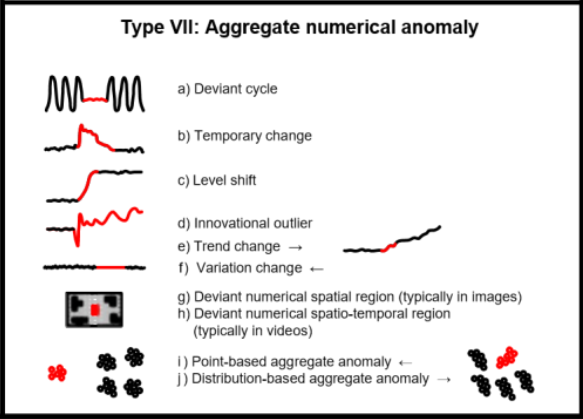
\includegraphics[scale=0.6]{Figures/series_anomaly}
	\decoRule
	\caption[Quantitative Anomalies]{Quantitative Anomalies \parencite{Foorthuis}}
	\label{fig:Anomaly_types}
	%https://arxiv.org/ftp/arxiv/papers/2007/2007.15634.pdf
\end{figure}

\subsection{Dataset Selection}
In the following subsections, it is proposed how and why the datasets are selected for the different experiments.

\subsubsection{1. Dataset}
The dataset, which should be used for the first experiment will be of synthetic nature. It consists of various cyclic patterns. In a second step, the dataset is enriched with anomalies. This way, two dataset are produced. The dataset without anomalies is used for an unsupervised learning approach whereas the dataset with labelled anomalies is used for a supervised approach. Comparing the two approaches should deliver some first insights on the abilities and learning behavior of the different neural network architectures.   

\subsubsection{2. Dataset}
The second dataset, which is used for anomaly detection, should consist of real data. To make sure, that the requirements, mentioned in section \ref{Problems of Existing Benchmarks} are met, the anomalies are embedded manually into the dataset. 

\subsubsection{3. Dataset}
As third dataset, one of the existing benchmark datasets should be used. Despite their obvious flaws, it is still considered useful to validate the previously achieved results on an official benchmark. Further, this gives insights into the overall usefulness of the proposed neural network architectures.

\subsection{Split of Dataset}
With all datasets the classical train, validation and test dataset approach is chosen. For the supervised approach, the training data is enriched with anomalies, whereas for the unsupervised approach a "clean" dataset is used. The final evaluation is done on a test dataset, which is the same for all approaches.


\section{Setup of Experiments}
The following section explains how the different experiments are conducted in detail. When desinging the experiments, the focus is put on comparability rather than optimally tuned neural networks.  Further, it is shown how the datasets and anomalies were engineered.

The following subsections give information on the chosen setups of the experiments that apply to all experiments, except where specifically stated otherwise.

\subsection{Supervised Learning}
The supervised learning approach refers to training the neural network on a labelled dataset. The dataset used for training already has the anomalies embedded. The task of finding the anomalies can also be described as a classification task, where the neural networks classifies a sequence as normal or anomalous. In such a case binary crossentropy and a sigmoid activation function are used as loss function and last layer activation fuction. The described loss 

\subsection{Unsupervised Learning}
The unsupervised learning approach refers to the training the neural network on a dataset that is free of anomalies. The neural network merely learns the cyclic pattern of the data. When learning the pattern the loss function applied is Mean Absolute Error (MAE), so the learning task is a regression. The actual anomaly detection hereby is done in a second step. As proposed in section \ref{CNN on univariate series}, the anomaly detector module calculates the Euclidean distance between predicted and actual value, where a large value corresponds to an anomaly.

\subsection{Neural Networks}

\subsubsection{Activation Function}
When designing the neural networks, as activation function "ReLu" (Rectified Linear Unit) is used. The function is non-linear and basically just returns the input if it is bigger than 0 and otherwise 0. This function is widely used, because of its simplicity and generally yields good results with little computation expenses.  

\subsubsection{Optimizer}
As optimizer, the often used default choice in machine learning, ADAM (Adaptive Moment Estimation), with the proposed default values, is applied \parencite{AUTHOR,YEAR}. ADAM update the learning rate when training making it faster than other optimizer such a Gradient Descent. On the downside, however, ADAM uses the memory for a given batch size and is found to generalize poorly in late stages of training.
%https://www.deeplearning.ai/ai-notes/optimization/ 

\subsection{Experiments}
In the following, it is suggested how the experiments on the 3 different datasets are conducted.

\subsubsection{1. Experiment}
In a first experiment the learning abilities of RNN and CNN are compared. It is investigated how useful the architectures are in a supervised and in an unsupervised setup. This experiment gives general insight on which setups and approaches work under which conditions. These insights are then investigated further in the second experiment.

\subsubsection{2. Experiment}
The second experiment is conducted on a more challenging dataset. Also the embedded anomalies are of a more challenging nature. The experiment delivers insight on what anomaly types can be detected with neural networks and which types are better to be detected with other (machine learning) approaches.

\subsection{Results}
As results three metrics are reported. First and most important, is the F1-Score which gives insight on the models ability to recognize anomalies. Second and third, the training and inference time are reported.



 